\paragraph{Drilling}

The \textbf{drilling} operation is performed by first picking up the drill handle from the instrument tray via the grabbing action (Figure \ref{fig::FeatureDrillingAttachments}).
Since drills are typically held in a number of different ways, the handgrip of the drill handle is adjustable.
Therefore, the virtual hand will not be displayed while holding the drill.
The instrument tray is located next to the operating table, where the patient's model will initially be positioned.
The drill handle initially has no attachment; users have to attach a drill bit first.

\begin{figure}[ht]
    \centering
    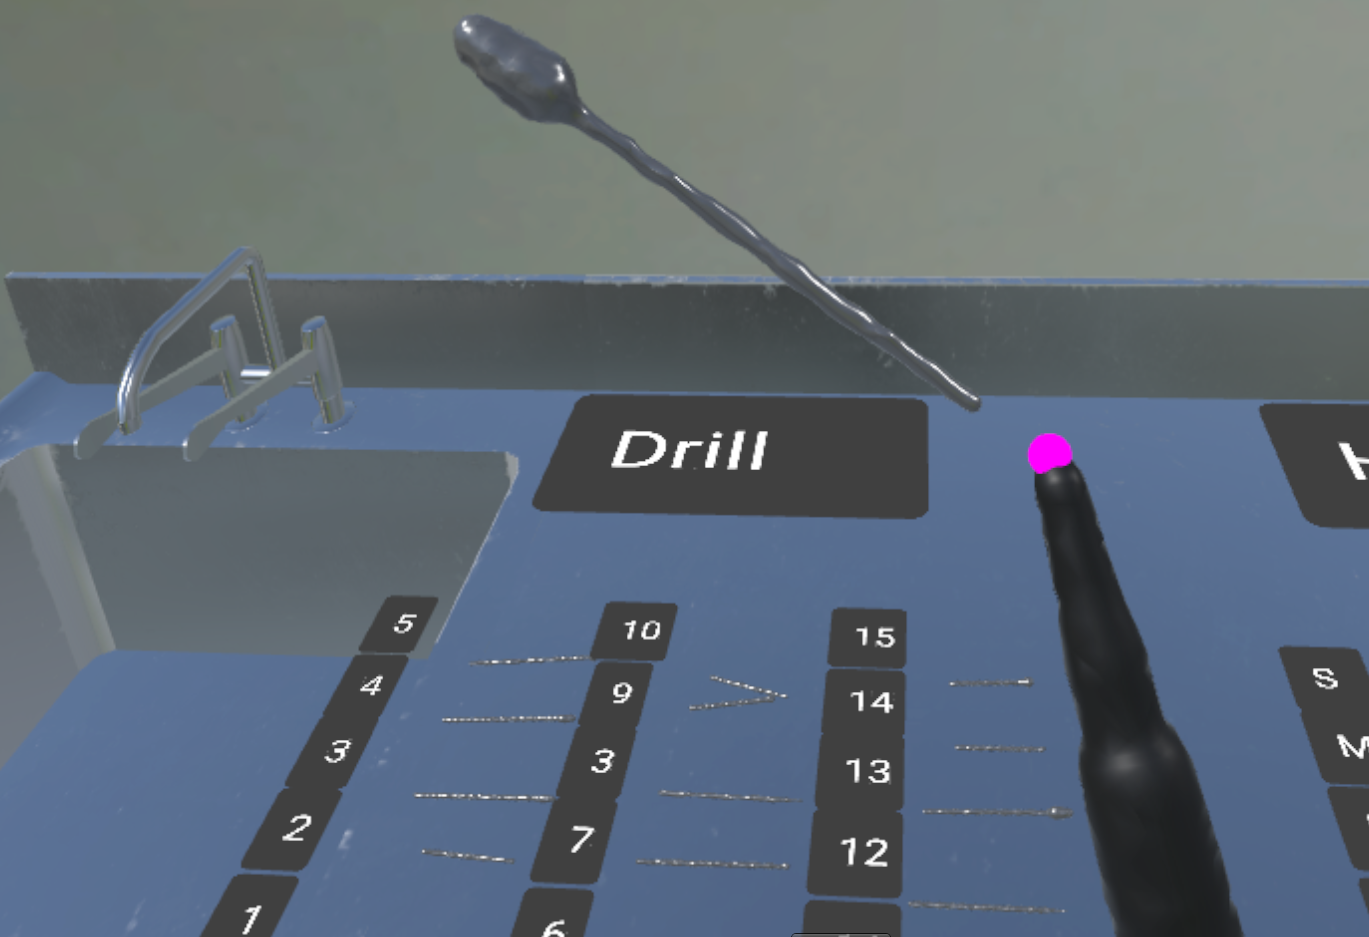
\includegraphics[width=\linewidth]{images/implementation/features/procedures/drilling_attachment.png}
    \caption{\label{fig::FeatureDrillingAttachments}Process of attaching drill bit to the drill handle. With the right hand, the user performs the indicate action by touching 
    the respective button. With the other hand, the drill bit is picked up by grabbing it and moved into the pink sphere to attach the bit.}
\end{figure}

In total, there are fifteen bits which can be used as an attachment for the drilling procedure.
Bits are modeled after their real counterparts in UHA.
They differ in size, length and width.
A visual signal is shown to the user while the indicate action is performed on the hand holding the drill handle.
By moving a drill bit to the visual indicator, the bit is attached to the handle (Figure \ref{fig::FeatureDrillingAttachments}).
Swapping out bits is performed by simply moving another bit into the indicator.
To perform the procedure, the drill handle must have a bit attached. 

\begin{figure}[ht]
    \centering
    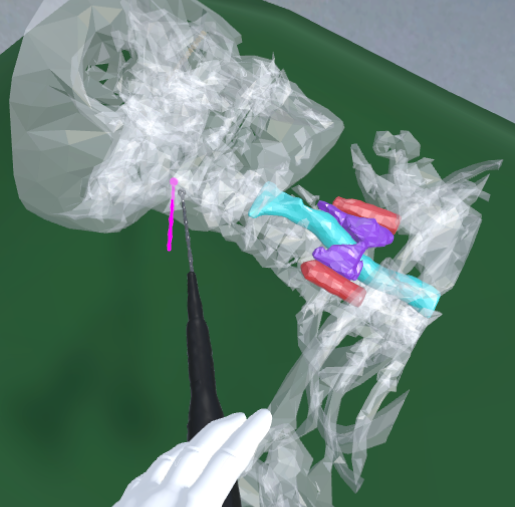
\includegraphics[width=\linewidth]{images/implementation/features/procedures/drilling.png}
    \caption{\label{fig::FeatureDrilling}Drilling procedure. The pink object represents the last performed step, which was performed using the drill by pressing 
    the perform button all the way.}
\end{figure}

By triggering the perform action of the hand holding the drill, a copy of the currently attached drill bit is created and added to the project case. 
This copy has a different material, i.e. a pink material, to indicate that it is part of the project case (Figure \ref{fig::FeatureDrilling}).
Additionally, textual information about the currently attached drill bit will be stored in the project case, so that the exact procedure can be reproduced later (Requirements \ref{req::N3}, \ref{req::N5}).
The drill bit will not be removed on performing a procedure, so that multiple drilling steps can be performed consecutively.
When the drill is no longer needed, it can either be placed back on the instrument tray or the operating table for quick access.
Note that any instrument, excluding the osteosynthesis plates described later, can be placed anywhere in the OT.